\documentclass{article}

\makeatletter
\renewcommand{\fnum@figure}{Εικόνα \thefigure}
\makeatother

\usepackage[greek, english]{babel}
\usepackage{alphabeta}
\usepackage{atbegshi, picture}

% Set page size and margins
% Replace `letterpaper' with`a4paper' for UK/EU standard size
\usepackage[letterpaper,top=2cm,bottom=2cm,left=3cm,right=3cm,marginparwidth=1.75cm]{geometry}

% Useful packages
\usepackage{amsmath}
\usepackage{graphicx}
\usepackage[colorlinks=true, allcolors=blue]{hyperref}
\usepackage[utf8]{inputenc}
\usepackage{indentfirst}

\newcommand\T{\rule{0pt}{2.6ex}}       % Top strut
\newcommand\B{\rule[-1.2ex]{0pt}{0pt}} 


\addto\captionsenglish{
  \renewcommand{\contentsname}
    {Περιεχόμενα}
}

% \title{Feasibility Study}
% \date{}

\begin{document}
% \maketitle

\begin{titlepage}
   \begin{center}
       \vspace*{1cm}

       \textbf{\huge Use Cases}

       \vspace{0.5cm}
        Τεχνολογία Λογισμικού
            
       \vspace{1cm}

       \textbf{Αγγελική Κούρου\\Κατερίνα Μητροπούλου\\Στεφανίδης Μάριος}
       
       \begin{figure}[!htb]
        \centering
        
\includegraphics[width=0.5\textwidth]{logo.png}
        \end{figure}
        
        \vspace{0.5cm}
        
        \begin{figure}[!htb]
        \centering
        \includegraphics[width=0.5\textwidth]{UoP.jpg}
        \end{figure}


       \vfill
            
       Τεχνικό Κείμενο για την Τεχνολογία Λογισμικού\\
            
       \vspace{0.5cm}
            
       CEID, ECE\\
       University of Patras\\
            
   \end{center}
\end{titlepage}



\noindent Η ομάδα μας

\begin{enumerate}
  \item Βεργίνης Δημήτριος, ΑΜ: 1066634 , ECE
  \item Βλαχογιάννης Δημήτριος, ΑΜ: 1067371, CEID
  \item Κούρου Αγγελική, ΑΜ: 1067499 , CEID
  \item Μητροπούλου Αικατερίνα - Quality Manager, ΑΜ: 1067409, CEID
  \item Στεφανίδης Μάριος - Project Manager, ΑΜ:1067458, CEID
\end{enumerate}

{
  \hypersetup{linkcolor=black}
  \tableofcontents
}

\newpage

\section{Εισαγωγή}

Τα Use Cases αποτελούν ένα σύνολο δραστηριοτήτων ή βημάτων που λαμβάνουν χώρα κατά την πλοήγηση ενός χρήστη (ή ρόλου, γνωστού στην UML ως ηθοποιού) σε ένα σύστημα, για να επιτευχθεί ένας στόχος. Ο ηθοποιός μπορεί να είναι άνθρωπος ή κάποιο άλλο εξωτερικό σύστημα. 
Για την ανάπτυξη ενός use case χρησιμοποιούνται τα διαγράμματα περιπτώσεων χρήσης, καθώς και λεκτική περιγραφή των περιπτώσεων αυτών.

\section{Διάγραμμα Περιπτώσεων Χρήσης}

Παρακάτω παρουσιάζεται το διάγραμμα περιπτώσεων χρήσης. Για την καλύτερη κατανόηση του διαγράμματος σημειώνεται ότι:

\begin{enumerate}
  \item Τα σκίτσα με τους ανθρώπους αντιστοιχούν στους ηθοποιούς του εκάστοτε use case, δηλαδή τους εμπλεκόμενους
  \item Οι μπλε ελλείψεις αντιστοιχούν στα use cases
  \item Οι μαύρες γραμμές απεικονίζουν άμεση συσχέτιση μεταξύ ενός ηθοποιού και μίας περίπτωσης χρήσης
  \item Οι μπλε διακεκομμένες γραμμές (το μπλε επιλέχθηκε για ευαναγνωσία) απεικονίζουν τη σχέση εξάρτησης μεταξύ δύο περιπτώσεων χρήσης, δηλαδή το use case στο οποίο δείχνει το βέλος δεν μπορεί να υπάρξει αν δεν έχει προηγηθεί το use case από το οποίο ξεκινάει το βέλος  
\end{enumerate}


\underline{Σημείωση}: Στο παρακάτω διάγραμμα, ενώ το use case που αφορά στην διαδικασία log in, είναι προαπαιτούμενο για την ύπαρξη όλων των υπολοίπων, δεν παριστάνονται οι συγκεκριμένες συσχετίσεις εξάρτησης για την καλύτερη παρουσίαση και ευαναγνωσία του διαγράμματος.

\newpage

\begin{figure}[!htb]
        \centering
        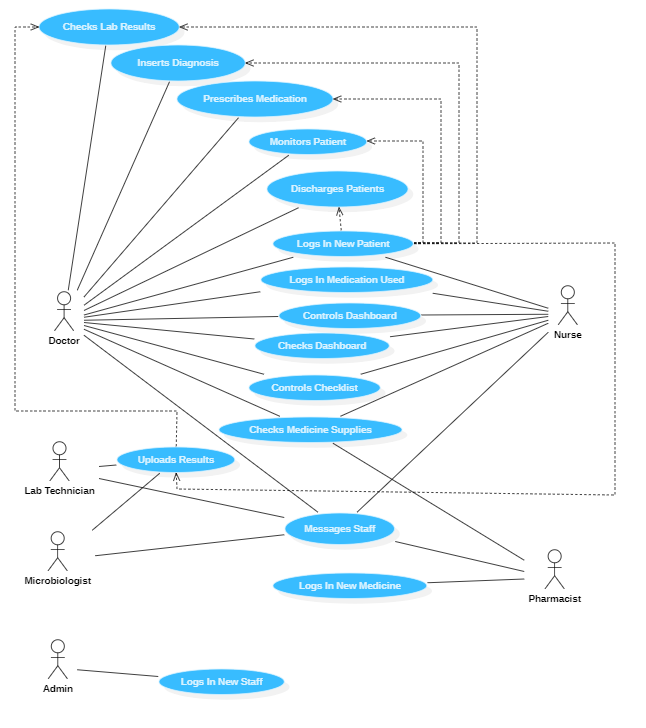
\includegraphics[width=1.1\textwidth]{UML.png}
        \caption{\label{fig: UML} Use Case Diagram}
\end{figure}
        
\vspace{0.5cm}

Για τις παρακάτω περιπτώσεις χρήσης δεν αναγράφονται στους πίνακες τα παρακάτω ως \par προαπαιτούμενα χάριν συντομίας:

\begin{enumerate}
    \item  Ο εκάστοτε "ηθοποιός" έχει καταχωρηθεί στο σύστημα
    \item Ο "ηθοποιός" έχει συνδεθεί στο \textbf{Medic World}
\end{enumerate}

\newpage

\section{Use Case 1: Ενέργειες στην Καρτέλα Ασθενούς}

Παρακάτω θα αναλυθεί το σενάριο χρήσης του \textbf{Medic World}, στο οποίο ένας γιατρός πραγματοποιεί συγκεκριμένες αλλαγές στην καρτέλα ενός ασθενούς.

\subsection{Γεική Περιγραφή}

Εξαιτίας του γεγονότος ότι οι λειτουργίες που μπορούν να πραγματοποιηθούν μέσω της καρτέλα του ασθενούς είναι πολυάριθμες, αποφασίσαμε να αναλύσουμε δύο απο τις πιο σημαντικές, την εισαγωγή διάγνωσης και την έκδοση εξιτηρίου.
\par Καθώς τα βήματα των συγκεκριμένων περιπτώσεων χρήσης ως ένα σημείο ταυτίζονται, στη συνέχεια θα παρουσιαστεί ένας κοινός πίνακας με τα βήματα που είναι ίδια και για τα δύο και στήν πορεία θα χωριστούν σε δύο διαφορετικά use cases. 

 \subsection{Γενικό Σενάριο Χρήσης}
 
 \begin{center}
     \begin{tabular}{|l|l|}
     \hline
      \textbf{Βήμα 1} & Ο γιατρός από το κεντρικό μενού επιλέγει να μεταφερθεί στις \T \\& καρτέλες των ασθενών \B \\
      \hline
      \textbf{Βήμα 2} &  Στο νέο παράθυρο εμφανίζονται όλοι οι ασθενείς που νοσηλεύονται στο νοσοκομείο \T\B \\
      \hline
      \textbf{Βήμα 3} & Στο ίδιο παράθυρο επιλέγει τον ασθενή που χρειάζεται διάγνωση \T\B \\
      \hline
      \textbf{Βήμα 4} & Σε νέο παράθυρο εμφανίζονται οι τρέχουσες ζωτικές ενδείξεις του ασθενούς, τις οποίες εξετάζει \T\B \\
      \hline
      \textbf{Βήμα 5} & Ο γιατρός επιθμεί να ελέγξει το ιστορικό του ασθενούς \T\B \\
      \hline
      \textbf{Βήμα 6} & Σε νέα καρτέλα εμφανίζονται τα δημογραφικά και κλινικά δεδομένα του \T\B \\
      \hline
      \textbf{Βήμα 7} & Στην συνέχεια, επιθυμεί να μελετήσει τα αποτελέσματα των εργαστηριακών \T \\& εξετάσεων του ασθενούς \B \\
      \hline
      \textbf{Βήμα 8} & Είναι έτοιμος να συμπληρώσει τη διάγνωση \T\B \\
      \hline      
     
     \end{tabular}
 \end{center}
 
\textbf{\underline{Εναλλακτική Ροή 1}:} \vspace{0.2cm}
\par \textbf{Βήμα 3.1.α:} Στην μπάρα αναζήτησης πληκτρολογεί το όνομα του ασθενούς και το σύστημα \par εμφανίζει προτάσεις με ασθενείς που είναι ήδη καταχωρημένοι και έχουν παρόμοιο όνομα με αυτό που \par πληκτρολογεί ο γιατρός.\vspace{0.1cm} 
\par Τα υπόλοιπα βήματα ταυτίζονται με τα βήματα 4 έως 8 της κανονικής ροής.

\vspace{0.2cm}

\par \textbf{Βήμα 3.1.β:}  Πληκτρολογεί το όνομα του ασθενούς και στην μπάρα αναζήτησης το σύστημα δεν \par εμφανίζει προτάσεις με ασθενείς που έχουν παρόμοιο όνομα με αυτό που πληκτρολογεί ο γιατρός. \vspace{0.1cm}
\par \textbf{Βήμα 4.1.β:} Το σύστημα εμφανίζει μήνυμα ότι δεν υπάρχει ασθενής με όνομα παρόμοιο με αυτό \par που αναζητεί ο γιατρός. \vspace{0.1cm}
\par \textbf{Βήμα 5.1.β:} Το σύστημα κλείνει την μπάρα αναζήτησης και εμφανίζει την οθόνη με τις καρτέλες \par των ασθενών. \vspace{0.1cm}

\par Τα υπόλοιπα βήματα ταυτίζονται με τα βήματα 4 έως 8 της κανονικής ροής. 
 
 \newpage
 
 \subsubsection{Εισαγωή Διάγνωσης}
 
 \begin{center}
     \begin{tabular}{|l|l|}
     \hline
      \textbf{Περίπτωση Χρήσης 1} & Ο γιατρός εισάγει τη διάγνωση ενός ασθενούς \T\B \\ 
      \hline
      \textbf{Ηθοποιός} & Γιατρός \T\B \\
      \hline
      \textbf{Σενάριο Περίπτωσης Χρήσης} & Ένας από τους ασθενείς χρείαζεται διάγνωση, οπότε \T\\& ο γιατρός εισέρχεται στην καρτέλα του, μελετάει τα\\& αποτελέσματα των εξετάσεών και τα συμπτώματά του και \\& καταλήγει σε διάγνωση \B \\
      \hline
      \textbf{Αφορμή} & Ασθενής χρειάζεται διάγνωση \T\B \\
      \hline
      \textbf{Προαπαιτούμενο 1} & Να έχει καταχωρηθεί ο ασθενής στο σύστημα \T\B \\
      \hline
      \textbf{Προαπαιτούμενο 2} & Να είναι έτοιμα τα αποτελέσματα των εργαστηριακών εξετάσεων \T\B \\
      \hline
     \end{tabular}
 \end{center}
 
 \begin{center}
     \begin{tabular}{|l|l|}
     \hline
      \textbf{Περιγραφή} & Αυτό το σενάριο περιγράφει μια κατάσταση όπου χρειάζεται \T \\& η πλοήγηση σε τέσσερις καρτέλες, οι οποίες τελικά\\& οδηγούν στην επίτευξη του στόχου. \B \\ 
      \hline
      \textbf{Βήμα 9} & Σε αναδυόμενο παράθυρο εμφανίζεται λίστα με πιθανές προτάσεις ασθενειών \T \\& που ταιριάζουν στο προφίλ του ασθενούς \B \\
      \hline
      \textbf{Βήμα 10} & Ο γιατρός επιλέγει κάποια από τις ασθένειες που ταιριάζει  \T\B \\
      \hline
      \textbf{Βήμα 11} & Επιβεβαίωνει την προσθήκη διάγνωσης \T\B \\
      \hline
      \textbf{Βήμα 12} & Σε αναδυόμενο παράθυρο εμφανίζεται μήνυμα επιτυχίας \T\B \\
      \hline    
      \textbf{Βήμα 13} & Επιλέγει την ένδειξη "ΟΚ" \T\B \\ 
      \hline
      \textbf{Βήμα 14} & Ενημερώνεται το σύστημα και το προφίλ του ασθενούς \T\B \\
      \hline
    \end{tabular}
 \end{center}
 
 \textbf{\underline{Εναλλακτική Ροή 1}:}  \vspace{0.2cm}
\par \textbf{Βήμα 10.1.:} Δεν τον ικανοποιεί καθόλου η λίστα των πιθανών ασθενειών, επομένως \par "κλείνει" αυτό το παράθυρο. \vspace{0.1cm}
\par \textbf{Βήμα 11.1:} Κατευθύνεται στο παράθυρο ολοκλήρωσης της διάγνωσης. \vspace{0.1cm}
\par \textbf{Βήμα 12.1:} Εισάγει τη διάγνωση του. \vspace{0.1cm}

\par Τα υπόλοιπα βήματα ταυτίζονται με τα βήματα 11 έως 14 της κανονικής ροής.

\vspace{0.2cm}

\textbf{\underline{Εναλλακτική Ροή 2}:}  \vspace{0.2cm}
\par \textbf{Βήμα 11.2:} Ο Γιατρός τροποποιεί την διάγνωση, εφόσον δεν τον ικανοποιεί πλήρως η πρόταση \par του συστήματος και επιθυμεί να συμπληρώσει κάτι επιπλέον. \vspace{0.1cm}

\par Τα υπόλοιπα βήματα ταυτίζονται με τα βήματα 11 έως 14 της κανονικής ροής.\vspace{0.1cm}
 
 \newpage
 
 \subsubsection{Έκδοση Εξιτηρίου}
 \begin{center}
     \begin{tabular}{|l|l|}
     \hline
      \textbf{Περιγραφή} & Αυτό το σενάριο περιγράφει μια κατάσταση όπου χρειάζεται \T \\& πλοήγηση σε τρεις καρτέλες. οι οποίες οδηγούν στην επίτευξη \\& του στόχου \B \\ 
      \hline
      \textbf{Βήμα 8} & Ο γιατρός συμπληρώνει τα απαραίτητα στοιχεία της φόρμας \T \\& εξιτηρίου (medication και nutrition recommendations) \\
      \hline
      \textbf{Βήμα 9} & Επιθυμεί να εκτυπώσει την συγκεκριμένη φόρμα \T\B \\
      \hline
      \textbf{Βήμα 10} & Σε αναδυόμενο παράθυρο εμφανίζεται το pdf αρχείο του εξιτηρίου \T\B \\
      \hline
      \textbf{Βήμα 11} & Δίνει έγκριση για την εκτύπωση και όταν αυτή ολοκληρωθεί, εμφανίζεται μήνυμα επιτυχίας \T\B \\
      \hline
      \textbf{Βήμα 12} & Επιστρέφει στο παράθυρο "Post-discharge Guidance" από το οποίο επιθυμεί να \T \\& κοινοποιήσει μέσω ηλεκτρονικού ταχυδρομείου τις οδηγίες εξιτηρίου \B \\
      \hline
      \textbf{Βήμα 14} & Σε νέο παράθυρο εμφανίζεται το εξιτήριο σε pdf μορφή από το οποίο \T\\&επιβεβαίωνει την κοινοποίηση του \B \\
      \hline
      \textbf{Βήμα 15} & Στέλνεται αυτομάτως μήνυμα στο email που έχει καταχωρηθεί για τον συγκεκριμένο ασθενή  \T\B \\
      \hline
      \textbf{Βήμα 16} & Επιστρέφει στο παράθυρο "Post-discharge Guidance" και επιβεβαίωνει την έκδοση του εξιτηρίου  \T\B \\   
      \hline
      \textbf{Βήμα 17} & Εμφανίζεται μήνυμα επιτυχίας και ενημερώνονται κατάλληλα οι νέες καρτέλες ασθενών  \T\B \\      
      \hline
     \end{tabular}
 \end{center}
 
 \vspace{0.2cm}


\vspace{0.3cm}

\textbf{\underline{Εναλλακτική Ροή 1}:} \vspace{0.2cm}
\par \textbf{Βήμα 15.1:} Δεν έχει καταχωρηθεί e-mail για τον συγκεκριμένο ασθενή, συνεπώς οδηγείται σε \par αναδυόμενο παράθυρο, το οποίο ζητά από τον γιατρό την συμπλήρωση κάποιας διεύθυνσης \par ηλεκτρονικού ταχυδρομείου. \vspace{0.1cm}
\par \textbf{Βήμα 16.1:} Γίνεται έλεγχος για την ορθότητα της διεύθυνσης του ηλεκτρονικού ταχυδρομείου \par που συμπλήρωσε.

\vspace{0.2cm}

\par \textbf{Βήμα 15.1.α:} Επιβεβαιώνει την καταχώρηση. \vspace{0.1cm}
\par \textbf{Βήμα 15.1.β:} Το email είναι λανθασμένο και το σύστημα κλειδώνει την λειτουργία επιβεβαίωσης \par καταχώρησης του email εώς ότου εισαχθεί το σωστό.

\par Τα υπόλοιπα βήματα ταυτίζονται με τα βήματα 16 και 17 της κανονικής ροής.\vspace{0.1cm}

\vspace{0.3cm}

\textbf{\underline{Εναλλακτική Ροή 2}:} \vspace{0.2cm}
\par \textbf{Βήμα 11.2/Βήμα 14.2:} Ο διαχειριστής επιθυμεί την ακύρωση της διαδικασίας.

\vspace{0.3cm}

\par \textbf{Βημα 12.2.α/Βήμα 15.2.α:} Εμφανίζεται νέο παράθυρο για την επιβεβαίωση της \par "ακύρωσης". \vspace{0.1cm}
\par \textbf{Βημα 13.2.α/Βήμα 16.2.α:} Επιβεβαιώνει την "ακύρωση". \vspace{0.1cm}
\par \textbf{Βημα 14.2.α/Βήμα 17.2.α:} Επιστρέφει στην προηγούμενη καρτέλα (post discharge guide) \vspace{0.3cm}

\par \textbf{Βημα 13.2.β/Βήμα 16.2.β:}  Απορρίπτει την "ακύρωση". \vspace{0.1cm}
\par \textbf{Βημα 14.2.β/Βήμα 17.2.β:} Επιστρέφει στην καρτέλα που βρισκόταν.
 
 \newpage
 
 \section{Use Case 2: Απασχόληση Χειρουργείου}
 
 Παρακάτω θα αναλυθεί το σενάριο χρήσης του \textbf{Medic World}, στο οποίο ένας χρήστης επιθυμεί να δηλώσει στο σύστημα τη χρήση ενός χειρουργείου.

\subsection{Περιγραφή}

\begin{center}
     \begin{tabular}{|l|l|}
     \hline
      \textbf{Περίπτωση Χρήσης 2} & Ο χρήστης δηλώνει την απασχόληση χειρουργείου \T\B \\ 
      \hline
      \textbf{Ηθοποιός} & Γιατρός \T\B \\
      \hline
      \textbf{Σενάριο Περίπτωσης Χρήσης} & Ένας γιατρός πρόκειται να εισάγει έναν ασθενή \T \\& σε κάποιο χειρουργείο και χρειάζεται να καταχωρηθεί\\& στην καρτέλα των χειρουργείων ότι το συγκεκριμένο\\& δωμάτιο δε θα είναι διαθέσιμο για κάποιο χρονικό διάστημα \B \\
      \hline
      \textbf{Ηθοποιοί} & Γιατρός, Νοσηλευτής \T\B \\
      \hline
      \textbf{Αφορμή} & Ασθενής χρειάζεται χειρουργείο \T\B \\
      \hline
      \textbf{Προαπαιτούμενο 1} & Να έχει καταχωρηθεί ο ασθενής στο σύστημα \T\B \\
      \hline
      \textbf{Πρoαπαιτούμενο 2} & Να έχει πραγματοποιηθεί διάγνωση του ασθενούς \T\B \\
      \hline
      \textbf{Προαπαιτούμενο 3} & Η διάγνωση να απαιτεί την εισαγωγή σε χειρουργείο \T\B \\
      \hline
     \end{tabular}
 \end{center}
 
 \subsection{Αναλυτικό Σενάριο Χρήσης}
 
 \begin{center}
     \begin{tabular}{|l|l|}
     \hline
      \textbf{Περιγραφή} & Αυτό το σενάριο περιγράφει μια κατάσταση όπου χρείαζεται \T \\& η πλοήγηση σε τρεις καρτέλες, οι οποίες οδηγούν στην \\& επίτευξη του στόχου. \B \\ 
      \hline
      \textbf{Βήμα 1} & Ο γιατρός από το κεντρικό μενού επιλέγει να μεταφερθεί στην \T \\& καρτέλα διαθεσιμότητας δωματίων \B \\
      \hline
      \textbf{Βήμα 2} & Επιθυμεί να ελέγξει την διαθεσιμότητα των χειρουργείων \T\B \\ 
      \hline
      \textbf{Βήμα 3} & Σε νέο παράθυρο εμφανίζονται όλα τα χειρουργεία \T \\& διαθέσιμα και μη με τις αντίστοιχες ενδείξεις \B \\
      \hline
      \textbf{Βήμα 4} & Ο γιατρός επιλέγει κάποιο από τα διαθέσιμα χειρουργεία \T\B \\
      \hline
      \textbf{Βήμα 5} & Σε νέα καρτέλα εμφανίζεται η φόρμα συμπλήρωσης των απαραίτητων στοιχείων \T\B \\
      \hline
      \textbf{Βήμα 6} & Για τη συμπλήρωση των στοιχείων όνομα ασθενούς, γιατρού και εγχείρησης \T \\& πληκτρολογώντας στο αντίστοιχο πεδίο κάθε φορά εμφανίζονται προτάσεις, \\& σύμφωνα με το κείμενο που πληκτρολογεί ο γιατρός \B \\
      \hline      
      \textbf{Βήμα 7} & Επιλέγει την ένδειξη "Done" για την ολοκλήρωση της διαδικασίας \T\B \\
      \hline
      \textbf{Βήμα 8} & Εμφανίζεται αναδυόμενο παράθυρο με την ένδειξη "Successful" \T\B \\
      \hline
      \textbf{Βήμα 9} & Ενημερώνεται το σύστημα και στην καρτέλα διαθεσιμότητας των χειρουργείων \T \\& εμφανίζεται πλέον ως μη διαθέσιμο το χειρουργείο που επέλεξε νωρίτερα ο γιατρός \B \\
      \hline
     \end{tabular}
 \end{center}
 
 \vspace{0.1cm}
 
\textbf{\underline{Εναλλακτική Ροή 1}:} \vspace{0.2cm} 
\par \textbf{Βήμα 6.1:} Πληκτρολογεί το όνομα του γιατρού και στην μπάρα αναζήτησης το σύστημα δεν \par εμφανίζει προτάσεις με γιατρούς που έχουν παρόμοιο όνομα με αυτό που καταγράφεται. \vspace{0.1cm}
\par \textbf{Βήμα 7.1:} Εμφανίζεται κατάλληλο μήνυμα αποτυχίας και δεν επιτρέπεται στον γιατρό να προχωρήσει \par με την διαδικασία, μέχρι να επιλέχθει κάποιο από το ονόματα που προτείνεται από τη λίστα.\vspace{0.1cm}
\par Εφόσον συμπληρωθούν τα κατάλληλα στοιχεία η τα βήματα της εναλλακτικής ροής ταυτίζονται με τα \par βήματα 7 εως 9 της κανονικής ροής.

\newpage

\textbf{\underline{Εναλλακτική Ροή 2}:} \vspace{0.2cm}
\par \textbf{Βήμα 6.2:} Ο γιατρός επιθυμεί την ακύρωση της \par διαδικασίας.

\vspace{0.2cm}

\par \textbf{Βήμα 7.2} Εμφανίζεται νέο παράθυρο για την επιβεβαίωση της  "ακύρωσης". \vspace{0.2cm}
\par \textbf{Βήμα 8.2.α:} Επιβεβαιώνει την "ακύρωση". \vspace{0.1cm}
\par \textbf{Βήμα 9.2.α:} Επιστρέφει στην προηγούμενη καρτέλα (λίστα χειρουργείων) \vspace{0.2cm}

\par \textbf{Βήμα 8.2.β:}  Απορρίπτει την "ακύρωση". \vspace{0.1cm}
\par \textbf{Βήμα 9.2.β:}  Επιστρέφει στην καρτέλα που βρισκόταν.

\section{Use Case 3: Καταχώρηση Νέου Φαρμάκου }
 
 Παρακάτω θα αναλυθεί το σενάριο χρήσης του \textbf{Medic World} κατά το οποίο ένας φαρμακοποιός επιθυμεί να εισάγει στο σύστημα ένα νέο φάρμακο.
 
\subsection{Περιγραφή}

\begin{center}
     \begin{tabular}{|l|l|}
     \hline
      \textbf{Περίπτωση Χρήσης 3} & Ο χρήστης εισάγει νέο φάρμακο στην καρτέλα προμηθειών \T\B \\ 
      \hline
      \textbf{Ηθοποιός} & Φαρμακοποιός \T\B \\
      \hline
      \textbf{Σενάριο Περίπτωσης Χρήσης} & Έχει γίνει από το νοσοκομείο αγορά ενός νέου φαρμάκου \T \\& και ο φαρμακοποιός καλείται να το καταχωρήσει \\& στην καρτέλα προμηθειών \B \\
      \hline
      \textbf{Αφορμή} & Η αγορά νέου φαρμάκου \T\B \\
      \hline
      \textbf{Προαπαιτούμενο 1} &  Να μην υπάρχει ήδη το φάρμακο στην καρτέλα προμηθειών \T\B \\
      \hline
     \end{tabular}
 \end{center}
 
 \subsection{Αναλυτικό Σενάριο Χρήσης}
 
 \begin{center}
     \begin{tabular}{|l|l|}
     \hline
      \textbf{Περιγραφή} & Αυτό το σενάριο περιγράφει μια κατάσταση όπου χρειάζεται \T \\& πλοήγηση σε δύο καρτέλες, οι οποίες οδηγούν στην επίτευξη \\& του στόχου \B \\ 
      \hline
      \textbf{Βήμα 1} & Ο φαρμακοποιός από το κεντρικό μενού επιλέγει να μεταφερθεί στην \T \\& καρτέλα των προμηθειών \B \\
      \hline
      \textbf{Βήμα 2} & Στο νέο παράθυρο επιλέγει την λειτουργεία "New Medicine" \T \\& (προσθήκη νέου φαρμάκου) \B \\
      \hline
      \textbf{Βήμα 3} & Σε νεό παράθυρο πληκτρολογώντας τη κατηγορία του φαρμάκου \T \\& στον χρήστη εμφανίζονται προτάσεις από τις υπάρχουσες κατηγορίες \\& (λ.χ. αντιβιοτικό), από τις οποίες μπορεί να επιλέξει κάποια \B \\
      \hline
      \textbf{Βήμα 4} & Στο ίδιο παράθυρο ο φαρμακοποιός καταχωρεί το όνομα του φαρμάκου \T\B \\
      \hline
      \textbf{Βήμα 5} &  Στο ίδιο παράθυρο συμπληρώνει τα τεμάχια που έχει προμηθευτεί το νοσοκομείο \T\B \\
      \hline
      \textbf{Βήμα 6} & Στο ίδιο παράθυρο καταγράφει τα όρια των τιμών που περιγράφουν την πληρότητα του \T \\& φαρμάκου (αν είναι σε αφθονία κ.ο.κ.)\B \\
      \hline
      \textbf{Βήμα 9} & Ολοκληρώνει τη διαδικασία καταχώρησης του φαρμάκου \T\B \\
      \hline
      \textbf{Βήμα 10} & Εμφανίζεται αναδυόμενο παράθυρο που υποδηλώνει την επιτυχία της διαδικασίας \T\B \\
      \hline    
      \textbf{Βήμα 11} & Γίνεται καταχώρηση στο σύστημα και στην καρτέλα διαθεσιμότητας φαρμάκων, \T \\& επιλέγοντας την κατηγορία  που αφορά το νεοεισαχθέν φάρμακο, εμφανίζεται \\& πλέον το νέο προϊόν \B \\
      \hline
     \end{tabular}
 \end{center}
 
 \newpage
 
\textbf{\underline{Εναλλακτική Ροή 1}:} \vspace{0.2cm} 
\par \textbf{Βήμα 3.1:} Η κατηγορία φαρμάκου που πληκτρολόγησε ο φαρμακοποίος δεν υπάρχει στο σύστημα, \par συνεπώς αυτομάτως δημιουργείται νέα κατηγορία.\vspace{0.1cm}

\par Τα υπόλοιπα βήματα ταυτίζονται με τα βήματα 4 έως 11 της κανονικής ροής.\vspace{0.1cm}

\vspace{0.2cm}
 
\textbf{\underline{Εναλλακτική Ροή 2}:} \vspace{0.2cm} 
\par \textbf{Βήμα 4.2:} Το φάρμακο που συμπλήρωσε ο φαρμακοποιός είναι ήδη καταχωρημένο, με αποτέλεσμα \par να μην του επιτρέπεται η συνέχεια της διαδικασίας εώς ότου διορθωθεί το όνομα ή κλείσει την καρτέλα.\vspace{0.1cm}

\par Εάν ο φαρμακοποιός συμπληρώσει διαφορετικό όνομα που δεν υπάρχει ήδη στο σύστημα, τότε τα \par υπόλοιπα βήματα ταυτίζονται με τα βήματα 5 έως 11 της κανονικής ροής.

\vspace{0.2cm}

\textbf{\underline{Εναλλακτική Ροή 3}:} \newline
\par \textbf{Βήμα 3.3/Βήμα 4.3/Βήμα 5.3/Βήμα 6.3:} Ο φαρμακοποιός επιθυμεί την ακύρωση της \par διαδικασίας.

\vspace{0.2cm}

\par \textbf{Βήμα 4.3/Βήμα 5.3/Βήμα 6.3/Βήμα 7.3:} Εμφανίζεται νέο παράθυρο για την επιβεβαίωση \par της  "ακύρωσης". \vspace{0.1cm}
\par \textbf{Βήμα 5.3.α/Βήμα 6.3.α/Βήμα 7.3.α/Βήμα 8.3.α:} Επιβεβαιώνει την "ακύρωση". \vspace{0.1cm}
\par \textbf{Βήμα 6.3.α/Βήμα 7.3.α/Βήμα 8.3.α/Βήμα 9.3.α:} Επιστρέφει στην προηγούμενη \par καρτέλα (φαρμακαποθήκη) \vspace{0.2cm}

\par \textbf{Βήμα 5.3.β/Βήμα 6.3.β/Βήμα 7.3.β/Βήμα 8.3.β:}  Απορρίπτει την "ακύρωση". \vspace{0.1cm}
\par \textbf{Βήμα 6.3.β/Βήμα 7.3.β/Βήμα 8.3.β/Βήμα 9.3.β:} Επιστρέφει στην καρτέλα που \par βρισκόταν.


\section{Use Case 4: Αποστολή Μηνύματος}

Παρακάτω θα αναλυθεί το σενάριο χρήσης του \textbf{Medic World}, στο οποίο χρήστες της εφαρμογής ανταλλάσσουν μηνύματα μεταξύ τους.

\subsection{Περιγραφή}

\begin{center}
     \begin{tabular}{|l|l|}
     \hline
      \textbf{Περίπτωση Χρήσης 4} & Ο χρήστης στέλνει μήνυμα σε κάποιον άλλο χρήστη της εφαμοργής \T\B \\ 
      \hline
      \textbf{Ηθοποιός} & Γιατρός \T\B \\
      \hline
      \textbf{Σενάριο Περίπτωσης Χρήσης} & Έχει εισαχθεί ένας νέος ασθενής στο νοσοκομείο και επιθυμεί να \T \\& μάθει, αν ένας συνάδελφός του έχει ελέγξει τις εξετάσεις \B \\
      \hline
      \textbf{Ηθοποιοί} & Γιατρός, Νοσηλευτής, Μικροβιολόγος, Υπεύθυνοι Εργαστηρίου, \T \\& Φαρμακοποιός, Διαχειριστής Συστήματος \T\B \\
      \hline
      \textbf{Αφορμή} & Έτοιμες εξετάσεις για έλεγχο \T\B \\
      \hline
      \textbf{Προαπαιτούμενο 1} & Να έχει εισαχθεί ο ασθενής στο σύστημα \T\B \\
      \hline
      \textbf{Προαπαιτούμενο 2} & Να έχει γίνει η παραγγελία των εξετάσεων \T\B \\
      \hline
      \textbf{Προαπαιτούμενο 3} & Να έχουν ολοκληρωθεί οι εξετάσεις \T\B \\
      \hline
     \end{tabular}
 \end{center}
 
\newpage

\subsection{Αναλυτικό Σενάριο Χρήσης}

 \begin{center}
     \begin{tabular}{|l|l|}
     \hline
      \textbf{Περιγραφή} & Αυτό το σενάριο περιγράφει μια κατάσταση όπου χρειάζεται \T \\& πλοήγηση σε τρεις καρτέλες, οι οποίες οδηγούν στην επίτευξη \\& του στόχου \B \\ 
      \hline
      \textbf{Βήμα 1} & Ο γιατρός από το κεντρικό μενού επιλέγει να μεταφερθεί στην \T \\& καρτέλα των μηνυμάτων \B \\
      \hline
      \textbf{Βήμα 2} & Επιθυμεί να συντάξει καινούργιο μήνυμα \T\B \\
      \hline
      \textbf{Βήμα 3} & Σε νέο παράθυρο πληκτρολογώντας το όνομα του χρήστη, εμφανίζονται προτάσεις \T \\& από τους ήδη εγγεγραμμένους χρήστες, από τους οποίους μπορεί να επιλέξει κάποιον  \B \\
      \hline
      \textbf{Βήμα 4} & Κατευθύνεται σε νέο παράθυρο στο οποίο εμφανίζεται η συζήτηση με τον \T \\& συγκεκριμένο χρήστη και οι διάφορες λειτουργίες αποστολής μηνύματος όπως \\& είναι η αποστολή φωτογραφίας, δημιουργία βιντεοκλήσης κ.ο.κ  \T\B \\
      \hline
      \textbf{Βήμα 5} &  Αποστέλλει το μήνυμα \T\B \\
      \hline
      \textbf{Βήμα 6} & Το σύστημα ενημερώνει τον χρήστη για την κατάσταση αποστολής του μηνύματος \T\B \\
      \hline
      \textbf{Βήμα 7} & Η κατάσταση του μηνύματος ενημερώνεται, αφού ο παραλήπτης το διαβάσει \T\B \\
      \hline
     \end{tabular}
 \end{center}
 
\vspace{0.2cm}
 
\textbf{\underline{Εναλλακτική Ροή 1}:} \vspace{0.2cm}
\par Ο χρήστης που επιθυμεί να συνομιλήσει, βρίσκεται ήδη στο ιστορικό των συζητήσεων του, επομένως: \vspace{0.05cm}
\par \textbf{Βήμα 3.1.α.:} Περιηγείται στην οθόνη και επιλέγει την συνομιλία τους.  \vspace{0.1cm}

\par Τα υπόλοιπα βήματα ταυτίζονται με τα βήματα 4 έως 7 της κανονικής ροής.\vspace{0.2cm}

\par \textbf{Βήμα 3.1.β:} Πληκτρολογεί το όνομα του χρήστη και στην μπάρα αναζήτησης το σύστημα δεν \par εμφανίζει προτάσεις με χρήστες που έχουν παρόμοιο όνομα με αυτό που πληκτρολογεί ο γιατρός. \vspace{0.1cm}
\par \textbf{Βήμα 4.1.β:} Εμφανίζεται μήνυμα αποτυχίας. 
\par \textbf{Βήμα 5.1.β.α:} Ο γιατρός πρέπει να πληκτρολογήσει εκ νέου ένα όνομα.\vspace{0.1cm}
\par \textbf{Βήμα 5.1.β.β:} Ο γιατρός πρέπει να αποχωρήσει από την καρτέλα.

\section{Use Case 5: Απομάκρυνση Απειλής από το Δίκτυο}

Παρακάτω θα αναλυθεί το σενάριο χρήσης του \textbf{Medic World}, στο οποίο ο διαχειριστής του συστήματος εντοπίζει μία απειλή στο δίκτυο και την αντιμετωπίζει.

\subsection{Περιγραφή}

\begin{center}
     \begin{tabular}{|l|l|}
     \hline
      \textbf{Περίπτωση Χρήσης 6} & Ο χρήστης διαχειρίζεται απειλές στο δίκτυο \T\B \\ 
      \hline
      \textbf{Ηθοποιός} & Διαχειριστής Συστήματος \T\B \\
      \hline
      \textbf{Σενάριο Περίπτωσης Χρήσης} & Έχει εντοπιστεί μία απειλή στο δίκτυο του νοσοκομείου \T \\& και ο διαχειριστής του συστήματος καλείται να την αντιμετωπίσει \B \\
      \hline
      \textbf{Αφορμή} & Εντοπισμός απειλής \T\B \\
      \hline
      \textbf{Προαπαιτούμενο 1} & Να εντοπιστεί περίεργη δραστηριότητα στο δίκτυο \T\B \\
      \hline
     \end{tabular}
 \end{center}

\newpage

\subsection{Αναλυτικό Σενάριο Χρήσης}

 \begin{center}
     \begin{tabular}{|l|l|}
     \hline
      \textbf{Περιγραφή} & Αυτό το σενάριο περιγράφει μια κατάσταση όπου χρειάζεται \T \\& πλοήγηση σε τέσσερις καρτέλες, οι οποίες οδηγούν στην επίτευξη \\& του στόχου \B \\ 
      \hline
      \textbf{Βήμα 1} & Ο διαχειριστής σύστηματος από το κεντρικό μενού επιλέγει να μεταφερθεί στo \T \\& μενού διαχείρισης δικτύου \B \\
      \hline
      \textbf{Βήμα 2} & Στο νέο παράθυρο επιθυμεί να ελέγξει τις συσκευές που είναι συνδεδεμένες στο δίκτυο \T\B \\
      \hline
      \textbf{Βήμα 3} & Σε νέο παράθυρο εμφανίζονται οι συσκευές που είναι συνδεδεμένες \T \\& στο δικτύο συνοδευόμενες από πληροφορίες όπως είναι το όνομα, ο \\& τρόπος σύνδεσης και οι IPv4 και MAC διευθύνσεις τους \B \\
      \hline
      \textbf{Βήμα 4} & Επιθυμεί να διαχειριστεί κάποια από τις συσκευές που εμφανίζονται \T\B \\
      \hline
      \textbf{Βήμα 5} & Σε αναδυόμενο παράθυρο εμφανίζονται περισσότερες λεπτομέρειες για την συσκευή \T\B\\
      \hline
      \textbf{Βήμα 6} & Ο διαχειριστής επιθυμεί να κατευθυνθεί στην καρτέλα διαχείρισης δικτύου \T\B \\
      \hline
      \textbf{Βήμα 7} & Οδηγείται σε παράθυρο που περιέχει τις ανεπιθύμητες MAC διευθύνσεις \T\B \\
      \hline
      \textbf{Βήμα 8} & Εισάγει τη MAC διεύθυνση της ανεπιθύμητης συσκευής στη λίστα \T\B \\
      \hline
      \textbf{Βήμα 9} & Ολοκληρώνει τη διαδικασία \T\B \\
      \hline
      \textbf{Βήμα 10} & Εμφανίζεται μήνυμα επιτυχίας \T\B \\
      
      \hline
     \end{tabular}
 \end{center}
 
\vspace{0.2cm}
 
\textbf{\underline{Εναλλακτική Ροή 1}:} \vspace{0.2cm}
\par \textbf{Βήμα 4.1:} Ο διαχειριστής κρίνει ότι η συσκευή δεν αποτελεί απειλή για το δίκτυο και η συσκευή \par πλέον δεν αναγνωρίζεται ως απειλή από το σύστημα.  


\section{Use Case 6: Καταχώρηση Νέου Μέλους του Προσωπικού}

Παρακάτω θα αναλυθεί το σενάριο χρήσης του \textbf{Medic World}, στο οποίο ο διαχειριστής του συστήματος προσθέτει ένα νέο μέλος εργατικό δυναμικό.

\subsection{Περιγραφή}

\begin{center}
     \begin{tabular}{|l|l|}
     \hline
      \textbf{Περίπτωση Χρήσης 8} & Ο διαχειριστής προσθέτει ένα νέο μέλος - χρήστη στο σύστημα \T\B \\ 
      \hline
      \textbf{Ηθοποιός} & Διαχειριστής Συστήματος \T\B \\
      \hline
      \textbf{Σενάριο Περίπτωσης Χρήσης} & Από το νοσοκομείο έγινε μία πρόσληψη ιατρικού προσωπικού και \T \\& ο διαχειριστής καλείται να τον προσθέσει στο σύστημα καθώς και \\& να δημιουργήσει τους κωδικούς του \B \\
      \hline
      \textbf{Ηθοποιοί} & Διαχειριστής Συστήματος \T\B \\
      \hline
      \textbf{Αφορμή} & Πρόσληψη γιατρού \T\B \\
      \hline
     \end{tabular}
 \end{center}

\newpage

\subsection{Αναλυτικό Σενάριο Χρήσης}

 \begin{center}
     \begin{tabular}{|l|l|}
     \hline
      \textbf{Περιγραφή} & Αυτό το σενάριο περιγράφει μια κατάσταση όπου χρειάζεται \T \\& πλοήγηση σε τρεις καρτέλες, οι οποίες οδηγούν στην επίτευξη \\& του στόχου \B \\ 
      \hline
      \textbf{Βήμα 1} & Ο διαχειριστής συστήματος από το κεντρικό μενού επιλέγει να μεταφερθεί στην \T \\& καρτέλα διαχείρισης εργαζομένων \T\B \\
      \hline
      \textbf{Βήμα 2} & Στο νέο παράθυρο εμφανίζονται οι διάφορες κατηγορίες εργαζομένων \T \\& (λ.γ. γιατροί, φαρμακοποιοί) \B \\
      \hline
      \textbf{Βήμα 3} & Επιλέγει τη κατηγορία γιατρών \T\B \\
      \hline
      \textbf{Βήμα 4} & Σε νέα οθόνη εμφανίζεται λίστα που περιέχει όλα τα μέλη του ιατρικού προσωπικού \T \\& (ενεργά και μη, με την αντίστοιχη ένδειξη) \B \\
      \hline
      \textbf{Βήμα 5} & Επιθυμεί να δημιουργήσει καινούργιο χρήστη σ' αυτή την κατηγορία \T\B \\
      \hline
      \textbf{Βήμα 6} & Σε αναδυόμενο παράθυρο που εμφανίζεται, συμπληρώνει το νέο username \T\B \\
      \hline
      \textbf{Βήμα 7} & Στο ίδιο παράθυρο επιλέγει τη λειτουργία "Generate New Password" και το σύστημα \T \\& δημιουργεί αυτόματα έναν ασφαλή κωδικό \B \\
      \hline
       \textbf{Βήμα 8} & Κατεθύνεται σε καίνουργιο παράθυρο για τη συμπλήρωση επιπλέον στοιχείων \T\B \\
      \hline
      \textbf{Βήμα 9} & Ολοκληρώνει τη διαδικασία και στην οθόνη εμφανίζεται η τελική μορφή της καταχώρησης\T\B \\
      \hline
      \textbf{Βήμα 10} & Επιβεβαιώνει την καταχώρηση \T\B \\
      \hline
     \end{tabular}
 \end{center}
 
 \vspace{0.2cm}

\textbf{\underline{Εναλλακτική Ροή 1}:} \vspace{0.2cm}
\par \textbf{Βήμα 6.1:} Το username που συμπλήρωσε ο διαχειριστής δεν πληροί τις προδιαγραφές και το \par σύστημα εμφανίζει ειδοποίηση για αλλαγή.\vspace{0.1cm}

\par \textbf{\underline{Σημείωση:}} Όσο ισχύει το βήμα 6.1 δε δίνεται στο διαχειριστή η δυνατότητα για δημιουργία κωδικού \par πρόσβασης.\vspace{0.1cm}

\par \textbf{Βήμα 7.1:} Ο διαχειριστής εισάγει διαφορετικό username που πληροί τις προδιαγραφές.\vspace{0.1cm}

\par Τα υπόλοιπα βήματα ταυτίζονται με αυτά τις κανονικής ροής (Βήμα 7-10).

\vspace{0.2cm}

\textbf{\underline{Εναλλακτική Ροή 2}:} \vspace{0.2cm}
\par \textbf{Βήμα 7.2/Βήμα 8.2/Βήμα 10.2:} Ο διαχειριστής επιθυμεί την ακύρωση της διαδικασίας.

\vspace{0.2cm}

\par \textbf{Βημα 7.2/Βήμα 8.2/Βήμα 10.2:} Εμφανίζεται νέο παράθυρο για την επιβεβαίωση της \par "ακύρωσης". \vspace{0.1cm}
\par \textbf{Βημα 8.2.α/Βήμα 9.2.α/Βήμα 11.2.α:} Επιβεβαιώνει την "ακύρωση". \vspace{0.1cm}
\par \textbf{Βημα 9.2.α/Βήμα 10.2.α/Βήμα 12.2.α:} Επιστρέφει στην προηγούμενη καρτέλα (λίστα \par ιατρικού προσωπικού) \vspace{0.2cm}

\par \textbf{Βημα 8.2.β/Βήμα 9.2.β/Βήμα 11.2.β:}  Απορρίπτει την "ακύρωση". \vspace{0.1cm}
\par \textbf{Βημα 9.2.β/Βήμα 10.2.β/Βήμα 12.2.β:} Επιστρέφει στην καρτέλα που βρισκόταν.

\vspace{0.2cm}

\textbf{\underline{Εναλλακτική Ροή 3}:} \vspace{0.2cm}
\par \textbf{Βήμα 8.3:} Ο διαχειριστής επιθυμεί να επιστρέψει στην προηγούμενη καρτέλα (username \& password) 

\newpage

\section{Use Case 7: Δημιουργία Post}

Παρακάτω θα αναλυθεί το σενάριο χρήσης του \textbf{Medic World}, στο οποίο ο γιατρός επιθυμεί να δημιουργήσει ένα post στο "Community Forum".

\subsection{Περιγραφή}

\begin{center}
     \begin{tabular}{|l|l|}
     \hline
      \textbf{Περίπτωση Χρήσης 8} & Ο γιατρός δημιουργεί ένα post στο Community Forum \T\B \\ 
      \hline
      \textbf{Ηθοποιός} & Γιατρός \T\B \\
      \hline
      \textbf{Σενάριο Περίπτωσης Χρήσης} & Ένας γιατρός στο νοσοκομείο επιθυμεί να κάνει μία ερώτηση \T \\& στο Forum σχετικά με μία συνάντηση που πρόκειται να \\& πραγματοποιηθεί στο νοσοκομειακό χώρο \B \\
      \hline
      \textbf{Ηθοποιοί} & Γιατρός, Νοσηλευτής, Μικροβιολόγος, Υπεύθυνοι Εργαστηρίου, \T \\& Φαρμακοποιός, Διαχειριστής Συστήματος \B \\
      \hline
      \textbf{Αφορμή} &  Ο γιατρός έχει μία απορία\T\B \\
      \hline
     \end{tabular}
 \end{center}

\subsection{Αναλυτικό Σενάριο Χρήσης}

 \begin{center}
     \begin{tabular}{|l|l|}
     \hline
      \textbf{Περιγραφή} & Αυτό το σενάριο περιγράφει μια κατάσταση όπου χρειάζεται \T \\& πλοήγηση σε τρεις καρτέλες, οι οποίες οδηγούν στην επίτευξη \\& του στόχου \B \\ 
      \hline
      \textbf{Βήμα 1} & Ο γιατρός από το κεντρικό μενού επιλέγει να μεταφερθεί στην \T \\& καρτέλα "Newsroom" \T\B \\
      \hline
      \textbf{Βήμα 2} & Στο νέο παράθυρο εμφανίζεται η καρτέλα "News Article" ως προεπιλογή \T\B \\
      \hline
      \textbf{Βήμα 3} & Επιλέγει την καρτέλα "Community Forum" \T\B \\
      \hline
      \textbf{Βήμα 4} & Σε νέα οθόνη εμφανίζονται όλα τα post που έχουν ήδη δημοσιευθεί, καθώς \T \\& και η δυνατότητα δημιουργίας νέας δημοσίευσης \B \\
      \hline
      \textbf{Βήμα 5} & Επιθυμεί να δημιουργήσει ένα καινούργιο post \T\B \\
      \hline
      \textbf{Βήμα 6} & Σε νέα καρτέλα εμφανίζονται όλες οι δυνατότητες επεξεργασίας δημοσίευσης,\T \\& όπως είναι η λήψη/προσθήκη φωτογραφίας, αναφορά σε κάποιο event κ.ο.κ. \B \\
      \hline
      \textbf{Βήμα 7} & Στο ίδιο παράθυρο συμπληρώνει το κείμενο και ολοκληρώνει τη δημοσιεύση \T\B \\
      \hline
       \textbf{Βήμα 8} & Ο γιατρός περιμένει για επιβεβαίωση της δημοσίευσης από τον διαχειριστή συστήματος \T\B \\
      \hline
       \textbf{Βήμα 9} & Η δημοσίευση εγκρίθηκε και "ανέβηκε" στο Community Forum \T\B \\
      \hline
     \end{tabular}
 \end{center}

\textbf{\underline{Εναλλακτική Ροή 1}:} \vspace{0.2cm}
\par \textbf{Βήμα 6.1/Βήμα 7.1:} Ο διαχειριστής επιθυμεί την ακύρωση της διαδικασίας.

\vspace{0.2cm}

\par \textbf{Βημα 6.1/Βήμα 7.1} Εμφανίζεται νέο παράθυρο για την επιβεβαίωση της \par "ακύρωσης". \vspace{0.1cm}
\par \textbf{Βημα 7.1.α/Βήμα 8.1.α:} Επιβεβαιώνει την "ακύρωση". \vspace{0.1cm}
\par \textbf{Βημα 8.1.α/Βήμα 9.2.α:} Επιστρέφει στην προηγούμενη καρτέλα ("Community Forum"). \vspace{0.2cm}

\par \textbf{Βημα 7.1.β/Βήμα 8.1.β:}  Απορρίπτει την "ακύρωση". \vspace{0.1cm}
\par \textbf{Βημα 8.1.β/Βήμα 9.1.β:} Επιστρέφει στην καρτέλα που βρισκόταν.

\textbf{\underline{Εναλλακτική Ροή 2}:} \vspace{0.2cm}
\par \textbf{Βήμα 9.2:} Η δημοσίευση δεν εγκρίθηκε από το διαχειριστή του στυστήματος. \vspace{0.1cm}
\par \textbf{Βήμα 10.2:} Λαμβάνει ειδοποίηση από τη λειτουργία "Messages". \vspace{0.1cm}
\par \textbf{Βήμα 11.2:} Ο γιατρός από το κεντρικό μενού επιλέγει να μεταφερθεί στην καρτέλα των μηνυμάτων. \vspace{0.1cm}
\par \textbf{Βήμα 12.2:} Επιλέγει τη συνομιλία με το όνομα \textbf{Medic World}. \vspace{0.1cm}
\par \textbf{Βήμα 13.2:} Σε νέο παράθυρο εμφανίζεται η συζήτηση με το λόγο που δεν εγκρίθηκε η δημοσίευση. \vspace{0.1cm}

\subsubsection{Use Case 8: Έγκριση Δημοσίευσης}

\begin{center}
     \begin{tabular}{|l|l|}
     \hline
      \textbf{Περίπτωση Χρήσης 8} & Ο διαχεριστής συστήματος καλείται να δώσει έγκριση \T \\& σε μία δημοσίευση που έχει δημιουργηθεί στο "Community Forum". \B \\ 
      \hline
      \textbf{Ηθοποιός} & Διαχεριστής Συστήματος\T\B \\
      \hline
      \textbf{Σενάριο Περίπτωσης Χρήσης} & ένας χρήστης της εφαρμογής επιθυμεί να δημοσιεύσει ένα post, \T \\&  το οποίο πρέπει να λλάβει έγκρισδη από το διαχειριστή συστήματος\B \\
      \hline
      \textbf{Αφορμή} &  έχχει δημιουργηθεί μία καινούργια δημοσίευση\T\B \\
      \hline
     \end{tabular}
 \end{center}

\subsection{Αναλυτικό Σενάριο Χρήσης}

 \begin{center}
     \begin{tabular}{|l|l|}
     \hline
      \textbf{Περιγραφή} & Αυτό το σενάριο περιγράφει μια κατάσταση όπου χρειάζεται \T \\& πλοήγηση σε τρεις καρτέλες, οι οποίες οδηγούν στην επίτευξη \\& του στόχου \B \\ 
      \hline
      \textbf{Βήμα 1} & Ο διαχεριστής συστήματος από το κεντρικό μενού επιλέγει να μεταφερθεί στην \T \\& καρτέλα "Newsroom" \T\B \\
      \hline
      \textbf{Βήμα 2} & Στο νέο παράθυρο εμφανίζεται η καρτέλα "News Article" ως προεπιλογή \T\B \\
      \hline
      \textbf{Βήμα 3} & Επιλέγει την καρτέλα "Community Forum" \T\B \\
      \hline
      \textbf{Βήμα 4} & Σε νέα οθόνη εμφανίζονται όλα τα post που έχουν ήδη δημοσιευθεί, η \T \\&  δυνατότητα δημιουργίας νέας δημοσίευσης και όλα τα post που βρίσκονται σε \\& λίστα αναμονής προς έγκριση  \B \\
      \hline
      \textbf{Βήμα 5} & Επιθυμεί να διαχειριστεί τα περιεχόμενα της λίστας με τα post που δεν έχουν ακόμη εγκριθεί\T\B \\
      \hline
      \textbf{Βήμα 6} & Σε νέα καρτέλα εμφανίζονται όλες οι δημοσιεύσεις που δεν έχουν "ανέβει" \T\B \\
      \hline
      \textbf{Βήμα 7} & Επιβεβαιώνει την κοινοποίηση κάποιας δημοσίευσης που πληροί τις προϋποθέσεις \T\B \\
      \hline
     \end{tabular}
 \end{center}
 
\textbf{\underline{Εναλλακτική Ροή 1}:} \vspace{0.2cm}
\par \textbf{Βήμα 7.1:} Δεν εγκρίνει την δημοσίευση. \vspace{0.1cm}
\par \textbf{Βήμα 8.1:} Αυτομάτως εμφανίζεται αναδυόμενο παράθυρο, στο οποίο μπορεί να προσθέσει το λόγο \par που δεν εγκρίθηκε το post. \vspace{0.2cm}

\par \textbf{Βήμα 9.1.α:} Επιλέγει επιβεβαίωση και η δημοσίευση δεν "ανεβαίνει" στο Community Forum. \vspace{0.2cm}

\par \textbf{Βήμα 9.1.β:}  Ο διαχειριστής επιθυμεί την ακύρωση της διαδικασίας.

\vspace{0.2cm}

\par \textbf{Βημα 10.1.β:} Εμφανίζεται νέο παράθυρο για την επιβεβαίωση της \par "ακύρωσης". \vspace{0.1cm}
\par \textbf{Βημα 11.1.β.α} Επιβεβαιώνει την "ακύρωση". \vspace{0.1cm}
\par \textbf{Βημα 12.1.β.α} Επιστρέφει στην προηγούμενη καρτέλα (Λίστα Αναμονής Έγκρισης) \vspace{0.2cm}

\par \textbf{Βημα 11.1.β.β}  Απορρίπτει την "ακύρωση". \vspace{0.1cm}
\par \textbf{Βημα 12.1.β.β} Επιστρέφει στην καρτέλα που βρισκόταν.

\newpage

\section{Use Case 9: Δημιουργία Εκδήλωσης}

Παρακάτω θα αναλυθεί το σενάριο χρήσης του \textbf{Medic World}, στο οποίο ο γιατρός επιθυμεί να δημιουργήσει εκδήλωση στο "Community Events".

\subsection{Περιγραφή}

\begin{center}
     \begin{tabular}{|l|l|}
     \hline
      \textbf{Περίπτωση Χρήσης 8} & Ο γιατρός δημιουργεί μία εκδήλωση στο "Community Events" \T\B \\ 
      \hline
      \textbf{Ηθοποιός} & Γιατρός \T\B \\
      \hline
      \textbf{Σενάριο Περίπτωσης Χρήσης} & Ένας γιατρός στο νοσοκομείο επιθυμεί να ενημερώσει το υπόλοιπο\T\\& προσωπικό σχετικά με μία εκδήλωση  που πρόκειται να πραγματοποι- \T\\&ηθεί στο νοσοκομειακό χώρο \B \\
      \hline
      \textbf{Ηθοποιοί} & Γιατρός, Νοσηλευτής, Μικροβιολόγος, Υπεύθυνοι Εργαστηρίου, \T \\& Φαρμακοποιός, Διαχειριστής Συστήματος \B \\
      \hline
      \textbf{Αφορμή} &  Ο γιατρός επιθυμεί να δημιουργήσει μία εκδήλωση\T\B \\
      \hline
     \end{tabular}
 \end{center}

\subsection{Αναλυτικό Σενάριο Χρήσης}

 \begin{center}
     \begin{tabular}{|l|l|}
     \hline
      \textbf{Περιγραφή} & Αυτό το σενάριο περιγράφει μια κατάσταση όπου χρειάζεται \T \\& πλοήγηση σε πέντε καρτέλες, οι οποίες οδηγούν στην επίτευξη \\& του στόχου \B \\ 
      \hline
      \textbf{Βήμα 1} & Ο γιατρός από το κεντρικό μενού επιλέγει να μεταφερθεί στην \T \\& καρτέλα "Newsroom" \T\B \\
      \hline
      \textbf{Βήμα 2} & Στο νέο παράθυρο εμφανίζεται η καρτέλα "News Article" ως προεπιλογή \T\B \\
      \hline
      \textbf{Βήμα 3} & Επιλέγει την καρτέλα "Community Events" \T\B \\
      \hline
      \textbf{Βήμα 4} & Σε νέα οθόνη εμφανίζονται όλα τα events που έχουν ήδη δημοσιευθεί, ξεχωριστά\T \\ & εμφανίζονται τα events που ο γιατρός έχει δηλώσει ενδιαφέρον καθώς  και η δυνατότητα\T \\& δημιουργίας νέας εκδήλωσης\B \\
      \hline
      \textbf{Βήμα 5} & Επιθυμεί να δημιουργήσει ένα καινούργιο event \T\B \\
      \hline
      \textbf{Βήμα 6} & Σε νέα καρτέλα ο γιατρός επιλέγει ότι η εκδήλωση θα διεξαχθή διά ζώσης\T \B\\
      \hline
      \textbf{Βήμα 7} & Σε νέο παράθυρο συμπληρώνει τις λεπτομέρειες για την εκδήλωση \T\B \\
      \hline
       \textbf{Βήμα 8} & Στη συνέχεια σε καινούργια καρτέλα επιλέγει την τοποθεσία της εκδήλωσης \T\B \\
      \hline
       \textbf{Βήμα 9} & Μέσω αναδυόμενου παραθύρου επιβλέπει την τελική μορφή της εκδήλωσης και επιλέγει τη\T\\& δημοσίευσή της \B \\
      \hline
       \textbf{Βήμα 10} & Στην καρτέλα "Community Events" εμφανίζεται η νέα εκδήλωση\T\B \\
      \hline
     \end{tabular}
 \end{center}

\textbf{\underline{Εναλλακτική Ροή 1}:} \vspace{0.2cm}
\par \textbf{Βήμα 6.1:} Ο γιατρός επιθυμεί η εκδήλωση να γίνει εξ αποστάσεως.\vspace{0.1cm}
\par \textbf{Βήμα 7.1:}  Σε νέο παράθυρο συμπληρώνει τις λεπτομέρειες για την εκδήλωση.\vspace{0.1cm}

\par \textbf{Βήμα 8.1.α:}  Σε νέα καρτέλα ο γιατρός επιλέγει ότι η εκδήλωση θα πραγματοποιηθεί μέσω του \par\textbf{Medic World}. \vspace{0.2cm}

\par \textbf{Βήμα 8.1.β:}  Σε νέα καρτέλα ο γιατρός επιλέγει ότι η εκδήλωση θα πραγματοποιηθεί μέσω άλλης \parεφαρμογής. \vspace{0.1cm}
\par \textbf{Βήμα 9.1.β:}  Σε αναδυόμενο παράθυρο ο γιατρός συμπληρώνει το link γιαα την εκδήλωση. \vspace{0.2cm}

\par Τα υπόλοιπα βήματα ταυτίζονται με τα βήματα 9 και 10 της κανονικής ροής. 

\newpage

\textbf{\underline{Εναλλακτική Ροή 2}:} \vspace{0.2cm}
\par \textbf{Βήμα 6.2/Βήμα 7.2/Βήμα 8.2/Βήμα 9.2:} Ο γιατρός επιθυμεί την ακύρωση της διαδικασίας.

\vspace{0.2cm}

\par \textbf{Βήμα 7.2/Βήμα 8.2/Βήμα 9.2/Βήμα 10.2:} Εμφανίζεται νέο παράθυρο για την επιβεβαίωση \parτης "ακύρωσης". \vspace{0.1cm}
\par \textbf{Βήμα 8.2.α/Βήμα 9.2.α/Βήμα 10.2.α/Βήμα 11.2.α:} Επιβεβαιώνει την "ακύρωση". \vspace{0.1cm}
\par \textbf{Βήμα 9.2.α/Βήμα 10.2.α/Βήμα 11.2.α/Βήμα 12.2.α:} Επιστρέφει στην αρχική καρτέλα \par(Community Events). \vspace{0.2cm}

\par \textbf{Βήμα 8.2.β/Βήμα 9.2.β/Βήμα 10.2.β/Βήμα 11.2.β:}  Απορρίπτει την "ακύρωση". \vspace{0.1cm}
\par \textbf{Βήμα 9.2.β/Βήμα 10.2.β/Βήμα 11.2.β/Βήμα 12.2.β:} Επιστρέφει στην καρτέλα που \parβρισκόταν.


\vspace{0.3cm}

\textbf{\underline{Εναλλακτική Ροή 3}:} \vspace{0.2cm}
\par \textbf{Βήμα 6.3/Βήμα 7.3/Βήμα 8.3/Βήμα 9.3:} Ο γιατρός επιθυμεί να μεταφερθεί σε προ- \parηγούμενη καρτέλα. \vspace{0.1cm}

\end{document}
